%!TEX encoding = UTF-8 Unicode
%%%%%%%%%%%%%%%%%%%%%%%%%%%%%%%%%%%%%%%%%%%%%%%%%%%%%%%%%%%%%%%%%%%%%%%%%%%
%%%%%%%%%%%%%%%%%%%%%%%%%%%%%%%%%%%%%%%%%%%%%%%%%%%%%%%%%%%%%%%%%%%%%%%%%%%
%%                          《合成生物学研究所》 模板                      %%       
%%                                                                       %%
%%                 modified from 《逻辑学研究》中文论文模板                %%
%%                                                                       %%
%%              中山大学逻辑与认知研究所逻辑学研究编辑部                     %%
%%                                                                       %%
%%                             Ver 1.31                                  %%
%%                                                                       %%
%%        You can modify it and distribute it freely    2014.06.04       %%
%%                                                                       %%
%%%%%%%%%%%%%%%%%%%%%%%%%%%%%%%%%%%%%%%%%%%%%%%%%%%%%%%%%%%%%%%%%%%%%%%%%%%

%-------------------------------------------------------------------------%
%
%  请以第一作者全拼为文件名另存此文档(后缀名仍为.tex),与 SLCN.sty 保存
%
%  在同一个文件夹中。你可能需要取消某些行首的注释符以添加需要的内容。
%  使用XeLaTex编译
%  参考文献的排版,请作者创建 .bib 文件, 并使用 BibTex 或者 Biber(有中文参考文献时) 进行排版。
%-------------------------------------------------------------------------%

%=========================================================================%
%                        一、编辑处理部分
%
%                  *** 作者请直接跳至第二部分 ***
%=========================================================================%

%-------------------------------------------------------------------------%
%    1.1 设定纸张大小、正文字体大小
%-------------------------------------------------------------------------%
\documentclass[b5paper,9pt,oneolumn,twoside,UTF8]{article}
\usepackage{SLCN}                                                         % 加载版面格式
\setmainfont{Times New Roman}

%-------------------------------------------------------------------------%
%    1.2 填入卷期号、出版年月
%-------------------------------------------------------------------------%
\newcommand{\myvolnumber}{x}                                              % 输入卷号
\newcommand{\myissnumber}{x}                                              % 输入当年期号
\newcommand{\mypubyear}{xxxx}                                             % 输入出版年份

%-------------------------------------------------------------------------%
%    1.3 填入起止页码、页数
%-------------------------------------------------------------------------%
\newcommand{\myfirstpage}{1}                                              % 输入起始页码
\newcommand{\mylastpage}{10}                                              % 输入终止页码
\newcommand{\mypages}{10}                                                 % 输入页数

%-------------------------------------------------------------------------%
%    1.4 填入收稿日期、修改稿日期
%-------------------------------------------------------------------------%
\newcommand{\receiveddate}{xxxx-xx-xx}                                    % 输入本文收稿日期
\newcommand{\revisiondate}{null}                                          % 预置修订日期为空,勿改此行
%\renewcommand{\revisiondate}{xxxx-xx-xx}                                 % 输入修订日期(若有)并取消该行注释

%-------------------------------------------------------------------------%
%    1.5 填入作者、单位英译名
%-------------------------------------------------------------------------%
\newcommand{\mysecondauthorEN}{null}                                      % 预置第二作者为空,请不要修改此行
\newcommand{\mythirdauthorEN}{null}                                       % 预置第三作者为空,请不要修改此行
\newcommand{\myfourthauthorEN}{null}
\newcommand{\myfifthauthorEN}{null}

\newcommand{\myfirstauthorEN}                                             % 请输入第一作者姓名
{First Author}

\newcommand{\myfirstaffiliationEN}{                                       % 请输入第一作者单位
\small{\it affiliation 1} \\
\small{\it another affiliation}
}

%\renewcommand{\mysecondauthorEN}{Second Author}                               % 若需要,请输入第二作者姓名,并取消该行注释
\newcommand{\mysecondaffiliationEN}{                                      % 若需要,请输入第二作者单位
\small{\it affiliation 2} \\
\small{\it another affiliation}
}

%\renewcommand{\mythirdauthorEN}{Third Author}                                % 若需要,请输入第三作者姓名,并取消该行注释
\newcommand{\mythirdaffiliationEN}{                                       % 若需要,请输入第三作者单位
\small{\it affiliation 3} \\
\small{\it another affiliation}
}

%\renewcommand{\myfourthauthorEN}{Fourth Author}
\newcommand{\myfourthaffiliationEN}{
\small{\it affiliation 4}
}


%\renewcommand{\myfifthauthorEN}{Fifth Author}
\newcommand{\myfifthaffiliationEN}{
\small{\it Affiliation 5}
}

%-------------------------------------------------------------------------%
%    1.6 填入文章类型
%  (original, bookreview, conferencereport)默认为original
%-------------------------------------------------------------------------%
\newcommand{\myarticletype}
{original}

\newcommand{\reviewbooktitle}                                             % 若文章为书评,请输入所评书的出版信息
{The information of the book reviewed by the author}

\newcommand{\reviewbooktitleEN}{null}                                     % 预置所评书的中译版为空,请勿修改此行
%\renewcommand{\reviewbooktitleEN}{中译版信息}                            % 若书有中译版,请输入中译版信息并取消该行注释

%-------------------------------------------------------------------------%
%    1.7 填入责任编辑
%-------------------------------------------------------------------------%
\newcommand{\myeditor}{
{\bf (责任编辑:某某某)}
}

%-------------------------------------------------------------------------%
%    1.8 缺省设置
%-------------------------------------------------------------------------%
\newcommand{\mysecondauthor}{null}                                        % 预置第二作者为空,请不要修改此行
\newcommand{\mythirdauthor}{null}                                         % 预置第三作者为空,请不要修改此行
\newcommand{\mygrants}{null}                                              % 预置“项目资助”为空,请不要修改此行
\newcommand{\mythanks}{null}                                              % 预置“致谢”为空,请不要修改此行


%=========================================================================%
%
%                        二、作者写作部分
%
%=========================================================================%

%-------------------------------------------------------------------------%
%    2.1 请填入论文题目、作者姓名、单位、电子邮箱
%-------------------------------------------------------------------------%
\newcommand{\mytitle}                                                     % 请输入论文题目
{底盘---回路耦合:合成基因回路设计新挑战}

\newcommand{\myrunningtitle}                                              % 请输入用于页眉的标题(可能需要缩短原来的标题)
{简短标题}

\newcommand{\myfirstauthor}                                               % 请输入第一作者姓名
{\kaishu 第一作者}

\newcommand{\myfirstaffiliation}                                          % 请输入第一作者单位,多个单位用 \\\small 分隔
{\small 单位1(到系所)}

\newcommand{\myfirstemail}                                                % 请输入第一作者电子邮箱
{\small xxxx@xxxx.xxx}

%\renewcommand{\mysecondauthor}{\kaishu 第二作者}                                 % 若需要,请输入第二作者姓名,并取消该行注释

\newcommand{\mysecondaffiliation}                                         % 若需要,请输入第二作者单位,多个单位用\\\small分隔
{\small 单位2(到系所)}

\newcommand{\mysecondemail}                                               % 若需要,请输入第二作者邮箱
{\small xxxx@xxxx.xxx}

%\renewcommand{\mythirdauthor}{\kaishu 第三作者}                                  % 若需要,请输入第三作者姓名,并取消该行注释

\newcommand{\mythirdaffiliation}                                          % 若需要,请输入第三作者单位,多个单位用\\small分隔
{\small 单位3(到系所)}

\newcommand{\mythirdemail}                                                % 若需要,请输入第三作者邮箱
{\small xxxx@xxxx.xxx}

\newcommand{\myfourthauthor}{null}

%\renewcommand{\myfourthauthor}{\kaishu 第四作者}
\newcommand{\myfourthaffiliation}{\small 单位四}

\newcommand{\myfourthemail}
{\small xxxx@xxxx.xxx}

\newcommand{\myfifthauthor}{null}

%\renewcommand{\myfifthauthor}{\kaishu 第五作者}
\newcommand{\myfifthaffiliation}{\small 单位五}

\newcommand{\myfifthemail}
{\small xxxx@xxxx.xxx}
%-------------------------------------------------------------------------%
%    2.2 请填入项目资助、致谢(选填)
%-------------------------------------------------------------------------%
%\renewcommand{\mygrants}{国家社会科学基金项目~XXXXXXXX}                  % 若需要,请输入项目名称及批号,并取消该行注释,多个项目以中文逗号分隔
%\renewcommand{\mythanks}{感谢XXX对本文的帮助。}                          % 若需要,请输入致谢内容,并取消该行注释

%-------------------------------------------------------------------------%
%    2.3 请填入中文摘要、关键词
%-------------------------------------------------------------------------%
   % 请在下面输入中文摘要

\newcommand{\myabstract}                                               
{随着合成生物学研究领域的发展以及对人工生命系统设计复杂程度的需求增加,合成基因回路设计呈现复杂化、规模化的发展趋势,导致合成基因回路行为变得难以预测。传统的基因回路设计框架注重回路内部元件作用关系的刻画和元件自身性能的参数调试,通过大量的试错,使回路功能达到次优化。近年来大量的工作表明,基因回路和底盘细胞存在难以避免的耦合:合成回路的基因表达受底盘细胞的资源调配机制调控,而合成基因回路的表达消耗底盘细胞的资源。这种相互作用往往导致底盘细胞生理状态的改变并影响回路功能。因此,将底盘细胞生理参数纳入到基因回路的设计框架中将有望提高基因回路设计的可预测性,提高理性设计能力。本文回顾了原核底盘细胞与基因回路的相互作用机制以及相关定量工作;同时,进一步总结了相关的生物物理模型如何帮助我们理解、预测和评估底盘---回路耦合带来的效应;最后介绍了通过基因回路正交化、模块化的方法减弱或规避底盘---回路耦合效应的最新进展,展现了它们对解决底盘---回路耦合效应的潜力。}
\newcommand{\mykeywords}                                                  % 请在下面输入中文关键词,以中文分号分隔
{大肠杆菌;合成生物学;系统生物学;底盘细胞;基因回路;相互作用;生物物理模型;正交化;模块化}

%-------------------------------------------------------------------------%
%    2.4 请填入英文标题、摘要(默认为null)
%-------------------------------------------------------------------------%
\newcommand{\mytitleEN}                                                   % 请输入英文标题
{Host-circuit Coupling: Toward a New Framework of Genetic Circuit Design}

\newcommand{\myabstractEN}                                                % 请输入英文摘要
%With the increasing complexity of genetic circuits, using traditional engineering principles to design genetic circuits has come to a bottleneck. Internal coupling between genetic circuits and the host cell alters the physiological state of the host and leads to unpredictable functions of the circuits. How to improve the predictablity of genetic circuits becomes a key question. In this review, we "summarizedthe mechanisms of interactions between the prokaryotic host cell and genetic circuits as well as the related quantitative works. Besides, the researches of reducing or avoiding the coupling effects by establishing mathematical models, orthogonalization and modularization are also reviewed.%
%英文摘要需要稍微展开一下
{With the burgeoning research area of synthetic biology and the extending complexity of artificial life systems, the behavior of large-scale genetic circuits becomes unpredictable. Traditionally, applying engineering discipline to genetic circuit design mainly focuses on the intrinsic parameters and interplay of the genetic parts, and tweaks circuits’ properties through extensive trial-and-error. Recent research shows an unavoidable coupling between circuits and host cell, which rises from the mechanism of the host's resource allocation while the expression depleting the host's building block and synthesis machine. This coupling changes the physiology states of the host and influences the functionality of circuits. Therefore, considering incorporate the host cells’ physiological states into genetic circuits design framework may improve the predictability of genetic circuits. In this review, we introduce the coupling mechanism between the prokaryotic host cell and genetic circuits, together with some related quantitative works. The attempts to predict or reduce the coupling effects by modeling, orthogonalization, and modular design are also summarized. }%
%-------------------------------------------------------------------------%
%    2.5 预置宏包和自定义命令(你可以补充需要的宏包和自定义命令)
%-------------------------------------------------------------------------%
\usepackage[pdfborder=0,CJKbookmarks=true]{hyperref}  % 使用内部超链接,其中第二个选项用于支持中文书签

\addbibresource{library.bib}				%填入参考文献库文件 .bib

%-------------------------------------------------------------------------%
%    2.6 打印标题页信息(作者请忽略此部分)
%-------------------------------------------------------------------------%
\begin{document}
\begingroup                                                               % 以下使得收稿日期以不加标记的脚注出现
\makeatletter
\let\@makefnmark\relax\footnotetext{
  \ifthenelse{\equal{\revisiondate}{null}}{{\bf 收稿日期:}\receiveddate}{
    {\bf 收稿日期:}\receiveddate;{\bf 修订日期:}\revisiondate
  }
}
\makeatother
\endgroup
\printtitlepage                                                           % 打印标题、作者、摘要等信息
%-------------------------------------------------------------------------%
%    2.7 正文内容从这里开始
%-------------------------------------------------------------------------%
\section{引言}
% 第一段总体性给出一个合成生物发展至今的成就
本世纪初两项创造性的工作,拨动开关\cite{Gardner2000}和压缩振荡子\cite{Elowitz2000},利用工程化的思想设计了人工基因回路并使其实现特定的生理功能。秉承这一思想,合成生物学在众多学科的交叉中诞生,在生命科学领域的研究中逐渐受到广泛的关注。近二十年来该学科出现许多重要的突破:一方面,通过对基因组的挖掘,人类得到大量定量刻画的生物元件\cite{Lou2012, Chen2013, Rudge2016},并设计出了越来越复杂的基因逻辑回路\cite{Bonnet2013, Nielsen2016},它们能响应特定的外界信号并输出预期的结果;另一方面,利用合成生物学工具,人类对生命系统的工作机理有了更深层次的认识,例如揭示细胞生长、分裂的普适机制\cite{Zheng2016,you2013};利用化学合成技术合成细胞基因组\cite{Zhang2017c, Hutchison3rd2016}为实现从头设计合成生命打下物质基础。另外,在产业方面,大量具有高价值的复杂产物通过合成基因回路实现了工业化生产,有希望取代传统化工合成,降低对环境的破坏和对化石能源的依赖性\cite{Luo2019, zhao2018a}。\\
% (这里有待展开讨论,并举些栗子)。
% 第二段点出目前遇到的挑战和本文的关注点
\indent 尽管如此,我们对基因的解读能力仍处在较低的水平:DNA序列提供的信息高度复杂,通过人工组合、设计的复杂基因回路放入到底盘细胞后,底盘细胞对特定信号的响应往往出乎我们的预期\cite{Zong2017, Gorochowski2017}。细胞在执行命令的过程中存在许多细节我们仍不清楚或难以定量描述的,但这些细节却也是基因回路功能实现的重要环节。基因回路同底盘之间存在种种联系,回路功能实现依赖细胞的DNA复制系统、转录和翻译系统以及各种代谢产物前体。不同的菌株、不同的生长条件,都会对基因的表达量产生影响\cite{10.15252/msb.20167402, 10.1038/nrmicro3238},而基因回路中不同基因的表达量决定了回路的输出结果;同时,外源的基因回路的表达对于底盘细胞而言是一种“负担”\cite{10.1038/s41467-020-18630-2, 10.1038/nmeth.3339},外源基因表达将占用有限的DNA、RNA、蛋白质的合成机器以及各种底物,这种资源上的占用将改变底盘细胞内源的基因表达,进而改变底盘细胞的生理状态。因此,基因回路和底盘细胞两者存在天然的耦合。然而长期以来,我们对合成基因的回路设计思路主要集中在单独元件的定量和预测上,忽略了底盘细胞与基因回路元件之间的影响。所以,使用特定条件下的单个基因模块的定量数据来预测不同工作背景下在基因回路的行为会出现偏差,导致合成基因回路设计不可避免的进入无限循环的“设计---构建---调试”中。不仅如此,许多工程菌,如环境治理工程菌、肠道菌群改造工程菌等,其工作环境往往不是标准的实验室条件,底盘细胞生理显然受环境的影响而发生了变化,导致很多基因回路无法实现预期功能\cite{cardinale2012contextualizing}。\\
% 第三段阐明挑战的细节和解决手段,只做简要描述
\indent 得益于系统生物学理论以及组学实验方法的发展,近年来,许多工作使得我们对于底盘细胞生理的理解有了更加全局、定量的认识\cite{hui2015, Gorochowski2017, Erickson2017}。将底盘细胞的生理状态纳入到对基因回路行为的理解中,许多反直觉的问题迎刃而解\cite{Boada2018};同时,这些理论也被应用到了合成基因回路设计的实践中,给合成基因回路设计带来了新的思路。除此之外,开发正交性元件和更加精巧的模块化设计也为解决这一问题提供了新的思路\cite{10.1016/j.copbio.2019.11.015}。本文将梳理近年来合成基因回路与底盘细胞相互耦合的理论研究,介绍底盘细胞与基因回路的相互作用,以及与之相关的定量技术,并进一步介绍近年来关于解开底盘-回路耦合的成果。 
\section{底盘细胞和基因回路的相互作用}
细胞通过一系列的生理生化过程从外界环境中摄取维持生长所需的物质,通过同化作用转化为提供复制、转录、翻译和酶促反应等生物过程所需的资源。在不同底盘细胞中,或者同一底盘在不同的环境和生长条件中,细胞会将其资源以不同的策略分配给不同的环节,以最大限度地提高其适应性\cite{Scott2010, you2013, hui2015, Zheng2020},分配策略的变化会导致回路的响应发生变化。同时基因回路作为外源基因,会竞争各种共享资源,如RNA聚合酶、核糖体和氨基酸,以及各种生化反应所需的酶和能量\cite{Borkowski2016, Towbin2017, 10.1038/msb.2012.70}对底盘细胞的生理状态产生影响,导致细胞生长缓慢、形态发生变化,这些变化同样作为基因回路的输入函数,影响基因回路行为,并可能产生难以预料的结果 \cite{10.1016/j.bpj.2017.12.010}。而且不同回路模块之间同样也存在竞争,这种竞争同样会导致回路的输出不符合预期(图\ref{fig.1} a)。本节我们将介绍关于回路-底盘相互作用的机制研究成果,并讨论这些机制带来的生理效应。
\subsection{底盘细胞对基因回路的影响}
\indent 不同生物底盘之间的基因背景差异会导致标准化的基因元件的输出结果的差异\cite{cardinale2013effects,vilanova2015standards},这为合成生物学的标准化设计提出了重大挑战。Moser等研究指出转化到不同\emph{Escherichia coli}菌株中的AND逻辑门会有出现不同的表现\cite{moser2012genetic}。同一培养条件下,AND 门回路在\emph{E. coli} DS68637中能够正常响应,而转入到 DH10B 菌株中却完全失去功能。而不同营养成分的培养基以及不同的培养条件也会对基因元件的响应产生改变 \cite{Liu2018a, 10.1038/s41586-020-2505-4, 10.15252/msb.20167402}。AND门在LB培养基中对诱导剂的响应非常灵敏;而转入贫瘠培养基后,诱导剂的加入甚至使细胞停止生长。\\
\indent 除了底盘细胞的遗传背景差异以及培养环境差异对基因回路造成的影响之外,底盘细胞的生长速率也是影响回路功能的关键因素之一。细胞中蛋白的降解主要以细胞生长的方式对胞内蛋白进行稀释\cite{Hintsche2013},因此的表达水平往往和底盘细胞生长速率相耦合,而蛋白表达水平的浓度高低则决定了基因线路的输出行为\cite{Bintu2005}。Tan等人分析了由自激活突变体T7 RNA聚合酶组成的基因回路,虽然该自激活过程是非协同的,但该回路的基因表达水平却呈现出双稳态。这一违反直觉的现象可以解释为,基因回路的表达引起了细胞生长速率的减慢,而同时细胞的生长对基因元件的表达存在着正反馈调节,进一步增加蛋白的积累,从而实现了双稳态现象\cite{Tan2009}。
\subsection{基因回路对底盘细胞的生长影响} % 生长压力 > 生长的影响
\indent 人工基因回路的表达占用了底盘细胞生长代谢相关的资源,影响细胞的正常生长\cite{10.1046/j.1365-2958.1996.5901313.x, 10.1093/nar/gkv1280}。外源基因回路对RNA聚合酶和核糖体\cite{Liu2018a}的竞争是导致这种压力的主要因素。当\emph{E. coli}细胞表达与生存不相关蛋白占细胞蛋白总量约30\%时,细胞会完全停止生长\cite{Vind1993, Scott2010}。除此之外,元件与底盘细胞的特异互作可能导致毒性,比如同代谢过程中的酶发生互作等。\\
\indent 另外,外源基因的表达甚至会引起底盘细胞的整体资源分配策略的改变。细胞本身存在动态调节分配策略的机制\cite{10.1016/j.molcel.2010.04.015, zhu2019growth, zhu2019ppGpp},(p)ppGpp(guanosine tetra- or penta-phosphate,鸟苷四(五)磷酸)转录翻译调节机制,当外源蛋白持续表达几代之后,\emph{E. coli}细胞可以利用(p)ppGpp的调控机制,实现对全局性资源的重新分配 \cite{10.1016/j.molcel.2010.04.015,  10.1038/s41564-019-0543-1}。较高的(p)ppGpp水平通过直接抑制核糖体合成以及蛋白翻译速度来抑制细胞生长。较低的(p)ppGpp水平限制参与细胞代谢相关蛋白的表达水平。在引入外源基因回路的条件下,外源基因对细胞内氨基酸资源的消耗,使得(p)ppGpp水平升高,降低核糖体的水平,提高代谢相关蛋白的表达量,这一策略在贫瘠培养基中可以有效协调细菌的资源分配。
\subsection{基因回路内部不同模块之间存在竞争}
\indent 基因回路中不同的模块之间也会竞争细胞资源\cite{Cookson2011a, 10.1016/j.bpj.2015.06.034, Wei2019, 10.1093/nar/gkaa734}。当一个外源回路中的基因都在争夺这些有限的资源时,基因之间就会产生非预期的相互作用。这些相互作用可以极大地改变基因回路的预期行为,导致实验结果与模型预测完全不符。例如,Qian等人的工作表明,当两个激活模块单独存在时,希尔函数可以很好的吻合实验结果。但是将两个模块串联形成更复杂的体系后,理论预测的结果甚至和实验结果完全相反\cite{Qian2017}。Wei 等人则建立了粗粒化的模型框架,用于描述生命体中转录因子、核糖体、蛋白降解酶等资源的竞争行为,通过统一的模型框架可以有效评估和理解基因回路中可能存在的竞争效应\cite{Wei2019}。\\
\indent 除了上述三种竞争效应外,底盘细胞和基因回路的互作还给带来了一系列其他效应,例如,增加同基因群体的异质性,降低遗传稳定性以及毒性效应。%该怎么自然过渡?
\subsection{基因回路导致底盘细胞生理异质性增强}
\indent 即使是相同基因型的细胞,在生长分裂等动态过程以及各种生理生化过程都存在噪声,造成了表型多样性 \cite{10.1103/physrevlett.114.078101, Wang:2011b4f, 10.1038/s41564-018-0161-3}。研究表明,这种差异往往随着生长速率的减小而变得显著\cite{Thomas2018, kim2020trade}。因此,外源基因的表达使得这种扰动变得更加明显,从而导致底盘细胞的生理异质性增强。而这种异质性导致一小部分表达量相对较低的细胞获得相对较快的生长速度。这类细胞便可以在不断的传代培养中取得优势,最终导致合成基因回路的失效\cite{Tan2009}(图\ref{fig.1} b)。另外,在细菌细胞中,资源的分配比例也可能会随着个体的差异而不同。例如,外源基因和底盘细胞基因往往公用\emph{E. coli}内源降解系统ClpXP,过量表达的蛋白可能导致不同蛋白的降解出现“排队效应”,这一随机的分配过程导致细胞的异质性增强\cite{Cookson2011a}。
% 是否要补充一下基因回路和底盘互作导致的双稳态行为?后面
\subsection{系统的遗传稳定性降低}
细胞的生长压力带来的负向筛选作用会减弱人工基因回路的遗传稳定性。研究表明基因回路功能可以给细胞带来很大的适应性劣势(fitness disadvantage)\cite{Sleight2013},并且发生适应性进化以减轻与表达外源蛋白质相关的代谢负荷或毒性。基因回路给底盘细胞带来压力同时导致底盘细胞生长速度往往低于野生型菌株,而突变导致的含有失效的基因回路的菌株往往具有更好的适应性,这样一来,在连续培养的过程中,带有期望功能的合成菌株会逐渐失去优势。Sleight等人\cite{Sleight2013} 评估了带有不同的调控元件的三种荧光蛋白在\emph{E. coli}中的遗传稳定性,发现表达量低和带有更少重复序列的基因回路具有更好的遗传稳定性(图\ref{fig.1} c)。重复序列容易导致基因重组进而导致序列丢失,因此有必要建立更大的优质元件库,减少元件在同一基因回路中的重复使用,使用低拷贝的质粒或者将基因回路整合到基因组也可以降低重组发生的概率\cite{10.1016/j.molcel.2016.06.006}。同时在设计的环节中加入同源序列检查的过程,避免元件组合的过程中产生意外的同源序列。% 把原先最后一个section糅合进了这一段。具有较少的基因,较低表达水平和较少重复DNA的基因回路表现出较高的进化稳定性\cite{Sleight2013}。高表达的基因回路往往带来更大的筛选压力,在这种进化压力下,细菌通常会选择通过失去功能的突变来逃避非必要表达的负担,从而使复制速度更快的突变细胞超越原始种群的生长。基因回路给底盘细胞带来压力同时导致底盘细胞生长速度往往低于野生型菌株,而突变导致的含有失效的基因回路的菌株往往具有更好的适应性,这样一来,在连续培养的过程中,带有期望功能的合成菌株会逐渐失去优势。因此提高基因回路在底盘细胞中的进化稳定性也是重要的话题。Sleight等人\cite{Sleight2013} 评估了带有不同的调控元件的三种荧光蛋白在大肠杆菌中的进化稳定性,发现表达量低和带有更少的重复序列的基因回路具有更好的进化稳定性。重复序列容易导致基因重组进而导致序列丢失,有必要建立更大的优质元件库,减少元件在同一基因回路中的重复使用,同时在设计的环节中加入同源序列检查的过程,避免元件组合的过程中产生意外的同源序列。
\subsection{基因回路导致的细胞的毒性}
在基因线回路的测试过程,往往会发现有些基因元件或回路会导致细胞形态发生变化,如纤维化。一般认为这种现象是由基因回路与细胞的一些生理过程发生了意外相互作用引起的。一种可能是,异源DNA中存在一些意外的功能序列。如,dnaA box 会严重影响细菌的分裂\cite{Kimelman2012};另外,富含AT序列的DNA序列可能是意外的启动子,高频的转录占用了细胞大量RNAP,造成RNAP不足\cite{Lamberte2017}。另外,外源基因的表达产物也可能与底盘细胞的基因组意外的互作,例如TetR家族中一些阻遏的蛋白异常调节底盘细胞的基因表达\cite{Stanton2014, Hasnain2019}。高表达dCas9也会严重影响细胞生理。组学实验发现dCas9蛋白在高表达水平下,能够非特异性结合到基因组上影响部分基因的转录水平 \cite{Cho2018}(图\ref{fig.1} d),导致细胞生长速率的急剧下降和细胞形态的纤维化。另外,也有实验表明gRNA只含有9碱基与目标位点匹配的情况下,也能有效结合到基因组上引起转录下调 \cite{Cui2018}。目前,还没有系统性的定量毒性的方法,对于这些意外的互作情况,使用组学技术,如RNA-seq等\cite{Liu2018a},可以有效地进行评估。\\
\indent 综上所述,基因表达与细胞生长之间存在着多方面的联系。对这些关系的认识可以提高对基因回路行为认识和预测,为合成基因回路的理性设计提供指导。基于上述实验证据,很多数学模型被用于描述这些机制,以进一步解释更复杂的生理现象。
\section{对合成基因回路与底盘细胞耦合效应的预测}
由于底盘细胞与基因回路之间存在复杂的相互作用,近年来不少工作利用数学模型解释了不同生长速度和药物作用下的细胞的行为\cite{Scott2010},将基因回路与底盘同时纳入到模型的框架中,使得许多基因回路失效的案例得到了解释,并为下一步底盘改造提供了方向。本节我们将介绍近年来出现的代表性的工作,介绍如何用生物物理模型去预测耦合效应。\\
\indent 近十几年来,随着合成生物学的发展,用生物物理模型描述回路与底盘的互作逐渐兴起,但模拟细胞内全部或主要生理过程的思想早在1979年就有报道\cite{Shuler1979}。从进入二十世纪以来,伴随着组学技术、生物定量技术的发展以及运算能力的提高,出现了全盘考虑所有已知生化过程的数学模型,其被称为全细胞模型(whole cell model)\cite{Tomita1999, carrera2015build, karr2012whole}。也有忽略大部分生化过程,仅考虑关键的几个生化过程的粗粒化的模型(coarse-grained model)\cite{Scott2010, Weiße2015,Liao2017}。 
\subsection{基于基因组的全细胞模型}
随着组学技术的兴起,构建全细胞模型的想法自然而然的产生,自2000年以来经历了构建全基因组网络结构、整合组学数据阶段\cite{Tomita1999},到目前拥有一定的预测能力。2012年,KarrJ等人基于多维组学数据对\emph{Mycoplasma genitalium}进行全细胞建模,将细胞的生理过程分为28个子过程并用16个细胞变量将子过程整合起来,并用合适的数学模型进行模拟,例如细胞代谢产物使用流平衡分析(Flux-balance Analysis, FBA)方法,蛋白等代谢产物降解采用泊松过程。在每个细胞周期内,每个子过程都在一个较短的时间尺度内独立模拟,并通过细胞变量整合。该模型可以对基因组各基因与转录因子之间的互作等诸多细胞行为做出预测,在这基础上通过对单基因扰动的模拟发现了已注释基因的新功能\cite{karr2012whole}。除了\emph{M. genitalium}以外,另一个比较成熟的生物模型是\emph{E. coli}模型,有研究以它为对象尝试建立对应全细胞模型,成功预测大部分基因或环境扰动对生长速度的影响,但实验数据的缺乏是该领域面临的很棘手的问题\cite{Carrera2014}。尽管如此,全细胞模型提供了一个从基因组到细胞生理动力学模拟的完整框架,因此,只需要通过修改或添加特定的子过程和细胞变量就可以实现预测,大大降低了模型构建的人力成本,比较适合进行基因模拟敲除、分子相互作用机理等理论预测工作。例如整合DnaA复制起始蛋白与基因组相互作用机制,预测了DNA复制时间(C期)同生长速率之间的关系,同实验数据进行比较,并进一步提出了关于 DnaA 结合位点同生长速率调控之间的关系\cite{Shuler2008}。有研究从全细胞模型出发关于噪音对基因开关的影响进行了研究,发现生长状态对噪音大小存在影响,由于转录翻译元件扩散速度慢和自我复制特性会产生正反馈机制,导致快速生长条件下的细胞存在更大的噪音\cite{Roberts2011}。通过在模型中加入基因线路模块,全细胞模型也可以进行基因线路动力学预测,Purcell 等人在回路噪音模拟问题上初步应用了\emph{M. genitalium}全细胞模型,再现了自抑制振荡回路中的噪音现象\cite{Purcell2013a}。\\
\indent 全细胞模型中涉及大量的参数,\emph{M. genitalium}的全细胞模型中整理了900篇文献中的1900个参数,包括分子和蛋白浓度、DNA蛋白质亲和力大小、RNA蛋白质降解速率、超螺旋程度影响等,以及更多当前无法定量的参数\cite{Babtie2017}。另外,繁杂的参数使得模型模拟结果与参数之间的关系变得难以解读。从“一切从简”的观点出发的粗粒化模型成为了与之互补的另一条途径。
\subsection{粗粒化模型}
粗粒化模型是希望通过一些简化模型,抓住所关注问题的核心机制,来对现象进行解释。早期细胞生理学家通过粗粒化模型想要回答的问题是,如何预测特定环境下的细胞生长速度。然而单纯从营养物质能量大小出发,无法解释实验结果,于是科学家们注意到前体代谢物对生长的关键作用以及蛋白质合成和底物之间的调节效应,相关内容总结于\cite{marr1991growth},这算是最初的粗粒化模型。而Scott等人基于实验现象,进一步将蛋白质组分为核糖体相关部分、代谢部分和其它部分,通过构建粗粒化模型得以解释实验中观察得到的现象\cite{Scott2010}。2015年Weiße等人又系统性地从能量角度整合Scott的研究结果并精简了相关因素,对细胞生长做出了更为准确的预测,并进一步讨论了其中回路与宿主之间的作用机制\cite{Weiße2015}。
2017年,Liao等人引入ppGpp作为全局调控因子,进一步对营养物质切换时细胞生长的实验现象进行了解释,并且引入了更多的竞争机制成功解释了基因回路相关的实验现象\cite{Liao2017}。粗粒化模型对细胞生理行为的描述越发准确,并且细胞与回路之间的互作也被越来越多的考虑到其中。\\
\indent 粗粒化模型的参数数量比全细胞模型的要少得多,Liao等人的关于\emph{E. coli}的粗粒化模型中的参数仅97个,实验测得有52个,其中部分参数相对稳定,不需要重复测量,可解释性和可实现性方面比全细胞模型更具有优势\cite{Liao2017}。\\
\indent 研究底盘---回路耦合效应,要抓住两者之间相互作用的关键节点,资源的竞争和全局性调度是绕不开的话题。根据不同的研究需要,抓住资源竞争过程中的瓶颈和底盘细胞相互作用的调节分子,研究人员构建了一系列模型帮助理解底盘---回路相互耦合的源头。外源基因回路的表达,对底盘细胞转录和翻译资源的竞争已经通过模型和实验得到了阐述,例如,Domitilla D. Vecchio 课题组和 J. Macía 课题组分别对宿主细胞内的不同基因基因线路资源竞争进行研究,提出了基因表达的“等成本曲线”模型,将RNA聚合酶资源和核糖体资源纳入到模型框架中,并成功地解释了实验现象\cite{10.1093/nar/gkv1280, 10.1016/j.bpj.2015.06.034}。另外,在资源较强的竞争条件下,随机性也会被放大,类似于“排队过程”。例如,蛋白翻译过程中不同种mRNA的丰度对有限核糖体结合竞争带来的基因表达波动\cite{Mather2013},类似的作用机制在转录、蛋白降解\cite{Cookson2011a}过程中都会用所体现,Wei 等人提出的分子竞争粗粒化模型为解释竞争过程在基因调控网络中的影响提供模型框架\cite{Wei2019}。\\
\indent 本质上,全细胞模型和粗粒化模型是两种不同的思考方向,全细胞模型是自下而上的逐一还原生化细节来构建完整细胞模型,而粗粒化模型是自上而下的对细胞进行简化。或许未来某个时刻这两条回路最终会到达一个终点,伴随着自动化实验技术的成熟,发展出一套成熟的细胞模型刻画体系,加快生物资源开发效率\cite{2018he}。
\section{减弱和规避合成基因回路与底盘细胞之间的耦合}
通过生物物理模型,可以帮助我们有效理解回路---底盘耦合的根源。减弱或者规避这种耦合可以大幅降低预测、构建大规模基因回路的难度。目前主要有两种思路,回路元件正交化\cite{Rackham2005}和设计模块化\cite{DelVecchio2015, Isaacs2004}。前者通过人工的改造和导入各个层次上的正交元件(包括正交DNA碱基,正交rRNA、tRNA、mRNA和正交蛋白质),来减弱甚至最终消除回路与细胞之间的耦合效应;后者通过基因互作拓扑结构的设计,来增强回路本身鲁棒性,减少其受宿主本身状态影响的效果。
% 光成功预测底盘细胞自身以及其与合成基因回路之间的互作还不足以解决这个问题,更进一步的我们需要减弱二者之间的耦合效应。
\subsection{合成基因回路正交化}
正交化希望实现维持回路其内部的逻辑调控的前提下,尽可能减少其内部元件与元件之间,以及元件与底盘细胞自身系统的不必要的交互。基因回路会不可避免地使用底盘细胞的各种资源,在特定情况下也需要建立与底盘细胞系统的接口,比如在进行天然产物的生产中,将对底盘细胞原有的代谢网络进行连接\cite{Martin2003, Atsumi2008}。正交化基因回路,减少了与底盘细胞的过多交互,则在进行模拟预测的时可以减少参数,提高系统的可预测性。通过在基因库中挖掘,正交化的DNA复制、转录、翻译系统也不断涌现出来,正交中心法则系统这一概念也被提出。正交中心法则系统希望中心法则中涉及的生物合成过程使用一套正交的系统完成,可以类比为计算机科学中虚拟机的概念 \cite{Liu2018b}。\\ % 当前,正交化的工作主要集中在对基因元件的正交设计中,通过对基因元件的定量测试和定向进化,
\indent 正交转录机器则早已在合成生物领域广泛使用,噬菌体RNA聚合酶是使用最多的元件,这类RNA聚合酶识别特定的启动子序列进行转录,大多为单体酶,且具有很强的转录活性。同时他们也容易被改造成为蛋白相互作用层次的逻辑门,例如对其结构域进行分割,融合其他类型的蛋白或结构域可以丰富其功能,例如,感光T7 RNAP\cite{Han2017, Baumschlager2017}。类似的,将 RNA 聚合酶与 DNA 识别结构域,锌指蛋白(ZFNs),转录激活因子(TALENs)或 CRISPR Cas蛋白等具有可设计能力的DNA识别蛋白进行融合表达,可以扩展其使用的范畴。例如,拓展理性化设计的启动子的转录动力学范围 \cite{McCutcheon2018}。另一类正交转录系统则基于 $\sigma$ 因子,利用不同来源的胞质外功能(Extracytoplasmic Function, ECF)$\sigma$ 因子对启动子序列的亲和性不同,通过共享RNA聚合酶核心酶库和不同家族的ECF $\sigma$ 因子对,可以设计出正交的ECF $\sigma$ 因子组合,实现在转录层面的绝缘\cite{rhodius2013}。蛋白的翻译涉及到大量复杂的生物过程,利用理性化和定向进化等手段,近年来,正交翻译体系也取得大量的进展。例如,改造氨酰tRNA合成酶可以将非天然氨基酸引入到蛋白的序列中,有希望给蛋白带来更多样的生理功能;得益于DNA合成成本的降低人工设计DNA序列替换细菌天然基因组,成功将\emph{E. coli}中64种密码子压缩到了61种,为扩充非天然氨基酸到合成生命的蛋白库打下了基础\cite{Fredens2019}。改变核糖体16S rRNA的序列,则可以得到正交核糖体,识别非典型的核糖体结合位点(Ribosomal Binding Site, RBS)序列,从而绝缘合成基因回路和底盘细胞的基因表达 \cite{Rackham2005, An2009a}。\\
% 完整的DNA正交复制系统应当可以在DNA---DNA聚合酶层面实现正交,即一种DNA聚合酶专门负责复制特定的DNA序列;例如,在酿酒酵母中,源自于\emph{Kluveromyces lactis} 的两个细胞质质粒能够利用相互独立的DNA聚合酶进行复制,通过基因工程改造,可以独立控制两个质粒的复制突变率 \cite{Ravikumar2014}。
% 例如,将T7 RNA聚合酶分割为两个部分,分别融合感光同源二聚蛋白结构域(VVD),可以使其在蓝光下形成二聚体从而激活转录 \cite{Han2017, Baumschlager2017}。
% 一个坑: 正交的转录因子 (尤其是阻遏蛋白) 的位置
% 正交降解系统
\indent 转录因子是合成基因回路设计中主要承担逻辑运算的元件,这类元件识别特定的序列激活或抑制下游基因的转录,未经正交化的转录因子存在交叉识别对应结合位点的风险。另外,结合到管家基因相关的DNA序列上可能影响细胞正常代谢,产生毒性。通过定向进化等手段对阻遏蛋白进行优化,增强其序列识别的特异性,也有助于降低细胞毒性\cite{Meyer2018}。除了典型的阻遏蛋白和激活蛋白外,许多具有识别序列功能的蛋白都可以通过理性化设计成为转录因子,如dCas9、TALENs等,由于上述的非特异性结合等原因,高表达此类蛋白往往给细胞带来较大的代谢压力。正交化设计的dCas9*\_Phlf在dCas9上引入了R1335K的突变,去除了dCas9的PAM(protospacer adjacent motif,前间区序列邻近基序)结合依赖性,并融合阻遏蛋白Phlf,使得它需要同时识别20碱基的sgRNA结合序列和30碱基的Phlf特异序列才能结合到DNA上,扩充了特异性结合序列的长度,降低了脱靶的风险,使细胞能耐受更高的表达量\cite{Zhang2018b}。
\subsection{模块化基因回路}
合成生物学的一大愿景是实现基因元件的即插即用\cite{endy2005foundations},即通过对基因元件的排列组合实现复杂的调控网络。传统的模块化主要是指元件模块化,即对启动子、编码序列、终止子等功能序列定义其边界,将他们独立出来。除了在元件设计过程中的模块化,更高层次的功能回路模块化方案最近备受关注。功能回路模块化将功能回路,例如逻辑门等,看作一个功能单元,通过合理的设计使每一个实现特定功能的回路的输入输出水平在插入到基因回路中时不受外部参数影响而发生变化\cite{10.1016/j.copbio.2019.11.015}。基因回路中各个功能模块之间的相互作用主要由转录因子来实现,而转录因子与下游模块的作用,例如结合到基因位点将导致游离转录因子浓度,进而扰动上游模块;对于底盘细胞而言,基因回路对转录翻译资源的消耗,将改变细胞生长速度以及各种资源库的总量,进而又影响了基因线中的各种动力学参数,这就产生了所谓的回溯效力(retroactivity)\cite{Qian2017},回溯效力的存在导致功能模块之间以及功能模块与细胞生理发生干扰,导致随着基因回路增加,功能模块的动力学属性发生变化。如何能够消除或规避回溯效力,实现回路的功能模块化呢?控制理论中反馈控制和非协同前馈环(Incoherent Feedforward Loop, iFFL)\cite{Mangan2003}为功能模块化提供了思路。在原先的功能模块中加入一个控制器,来执行反馈调节功能或与原先模块组成一个非协同前馈环,在一定程度上解决了这一问题。\\
% 当前大量基于反馈控制的解决方案已经被应用到基因回路的设计上,Vecchio 等人总结为三个层次:全局水平,局部水平和宿主偏好水平(host-favoring)。
\indent 负反馈调节可以使基因回路的稳态输出水平仅与自生元件的动力学性质决定,而不受基因表达生成和稀释速率影响。当前大量基于反馈控制的解决方案已经被应用到基因回路的设计上,可以归结为局部水平和全局水平两类(图\ref{fig.3})。\\
\indent 局部水平的反馈策略主要着眼于功能模块输出本身的稳定性,希望利用负反馈系统来隔离模块与模块之间,以及模块与底盘细胞之间的相互影响\cite{Shopera2017,huang2018}。例如,使用转录后调控元件sRNA形成负反馈环,使每一模块的稳态表达水平都得以固定,使得它们对来自资源竞争产生的扰动具有抵抗的能力(图\ref{fig.3} b)\cite{huang2018}。类似地,Aoki等人则采用了对偶积分反馈的策略,在保证了模块的抗扰动能力的同时,实现了模块稳态输出的可调性(图\ref{fig.3} c)\cite{Stephanie2019}。\\
\indent 基于全局的资源调控反馈策略能够根据基因回路表达带来的负担对所需的资源进行调控。这样的模块化策略还可以与正交系统联用。例如,正交核糖体基因表达系统中加入反馈控制模块,能够实现对正交核糖体与内源核糖体比例的动态分配,使正交核糖体的比例按需分配给基因回路,减轻基因回路内部的资源竞争带来的耦合(图\ref{fig.3} e)\cite{Darlington2018}。\\
\indent 另一种反馈策略则由宿主生理状态决定,根据代谢压力的大小来决定外源基因的表达。通过实验筛选出外源基因高表达时转录水平上调的启动子,利用这类启动子激活下游基于dCas9的转录抑制系统, 从而确保外源基因回路对细胞的压力维持在一个较低的水平(图\ref{fig.3} d) \cite{ceroni2018burden}。\\
\indent 正反馈回路虽然无法使模块的输出水平更加稳定,但也有独特的用处。在代谢工程领域,为了增强基因回路的遗传稳定性,会利用与生理状态偶联的正反馈回路(图\ref{fig.3} f),这一策略使得表达目的产物的个体具有生长优势\cite{Rugbjerg2018, Xiao2016}。\\
\indent 除了反馈环这一策略外,另一种基于转录调控的模块化手段则采用了非协调前馈环,Segall-Shapiro等人通过对iFFL模体的分析,指出当iFFL模体中阻遏蛋白无协同效应时,稳态下模体的输出将为一个常数而不依赖基因的拷贝数、细胞生长速度,通过这一简单的策略,可以使基因在不同拷贝数下实现稳定表达(图\ref{fig.3} g) \cite{Segall-Shapiro2018}。
\section{总结与展望}
过去20年来,合成生物学领域涌现出了大量创造性的工作,证明了利用合成生物学理论、方法改造生命为人类所用的可行性。未来,合成基因回路需要能够适应更多的遗传背景迥异的底盘细胞,以及更加复杂多变的使用环境。然而,由于我们对底盘细胞缺乏更系统、全面的认识,导致更为复杂的人工生命系统的开发工作效率低下。本文总结了当前关于细胞生理定量,底盘细胞与底盘细胞相互耦合的机制,以及如何避免因耦合引起的基因回路失效等方面的研究进展。我们认为在未来应当注重:1.更加系统、定量化的底盘细胞生理研究,理清底盘细胞在各种条件下,如逆境、非稳态,的资源调控机制,扩大研究的底盘细胞的种类;2.挖掘、定量、优化更多的正交基因调控元件,阐明不同遗传背景的底盘细胞基因元件的性能;3.开发更加精准、高通量的定量手段,利用多层次的组学技术,为定量刻画底盘细胞---基因回路相互作用机制提供更加可靠、全面的数据;4.建立更加精准的模型预测框架,包括:将底盘细胞与回路的模型描述整合在一起,增强基因回路行为的可预测性;以及从DNA序列生成环节出发,检查序列组合中意外产生的功能序列,如dnaA结合序列、启动子、转录因子结合序列等;5.规避“非预期”的底盘细胞与基因回路相互作用的解决方案,如利用反馈控制机制设计更加模块化的基因回路。
\newpage
\begin{figure}[H]
  \centering
  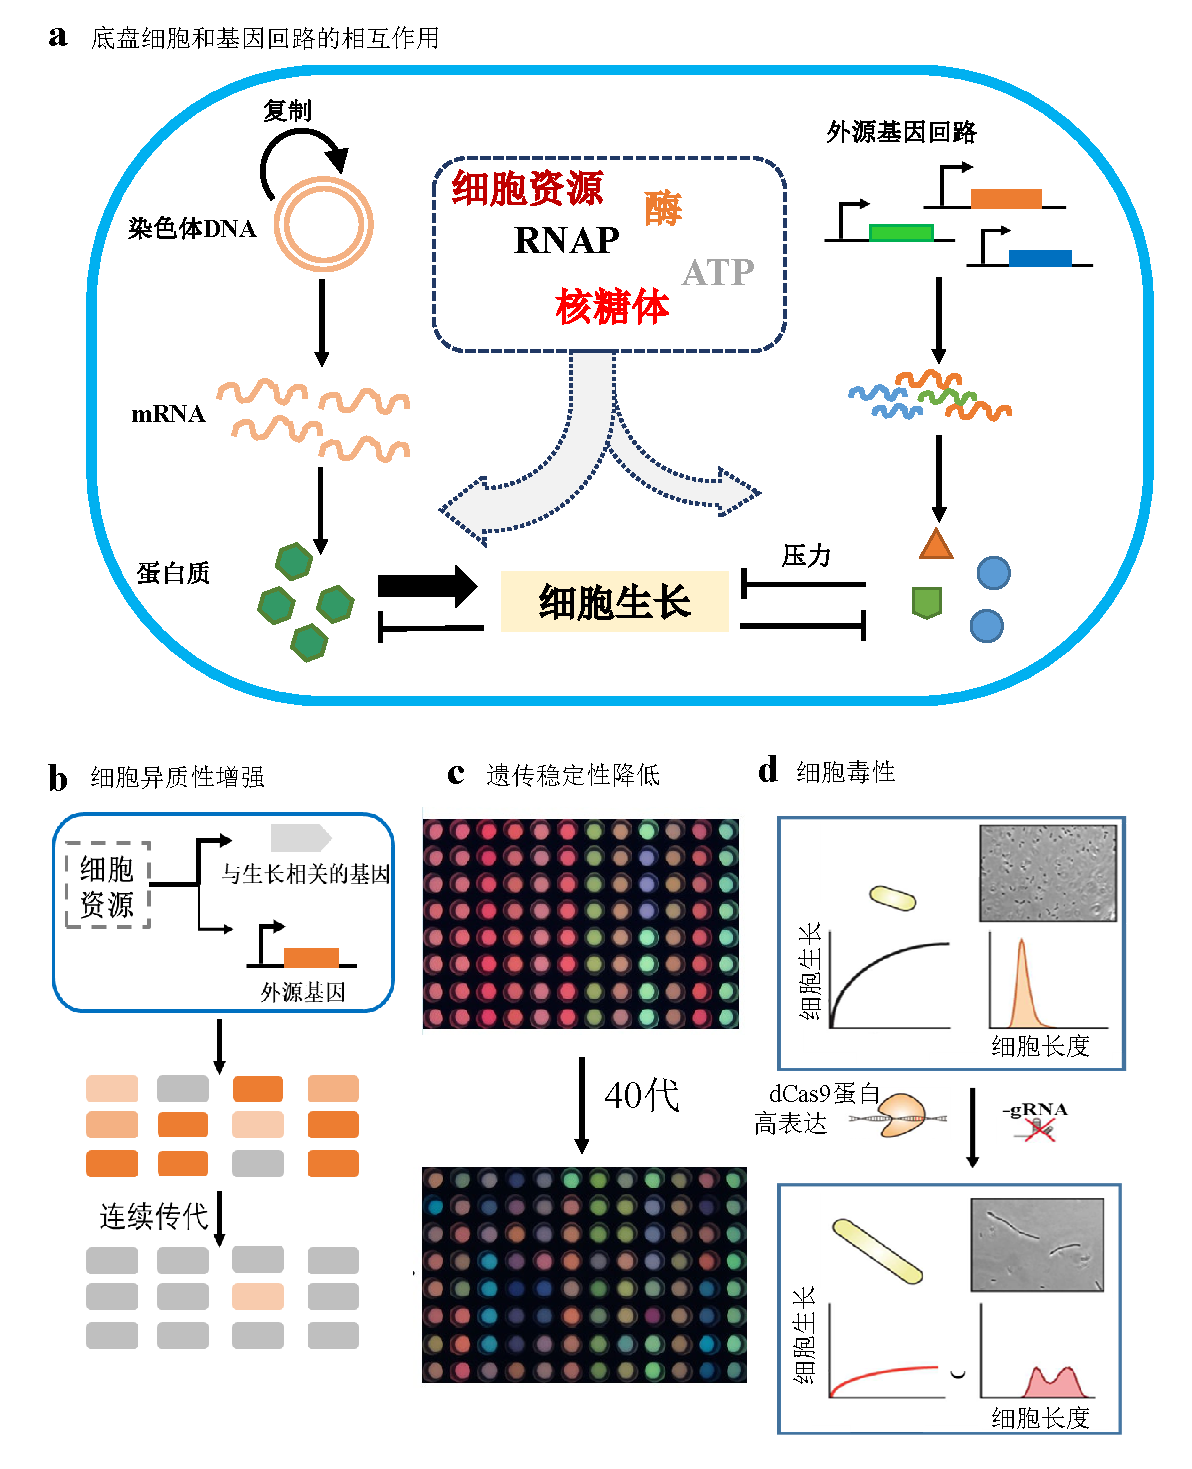
\includegraphics[width=1.0\textwidth]{reviewer_figure1}
  \caption{底盘细胞和基因回路之间的相互作用。{\scriptsize (a)底盘细胞和外源基因回路通过竞争细胞内的资源实现耦合,这种相互作用带来了一系列的效应:(b)细胞异质性增强:外源基因的表达存在差异性,导致细胞异质性增强,一小部分表达量相对较低的细胞获得相对较快的生长速度,这类细胞便可以在不断的传代培养中取得优势,最终导致合成基因回路的失效;(c)遗传稳定性降低(图修改自\cite{Sleight2013}):将带有不同的调控元件的三种荧光蛋白随机组合进行连续培养发现,表达量低和带有更少重复序列的基因回路具有更好的遗传稳定性;(d)细胞毒性(图修改自\cite{Hasnain2019}):dCas9蛋白在高表达水平下,能够非特异性结合到基因组上影响部分基因的转录水平,导致细胞生长速率的急剧下降和形态纤维化。}}
  \label{fig.1}
\end{figure}
\begin{figure}[H]
  \centering
  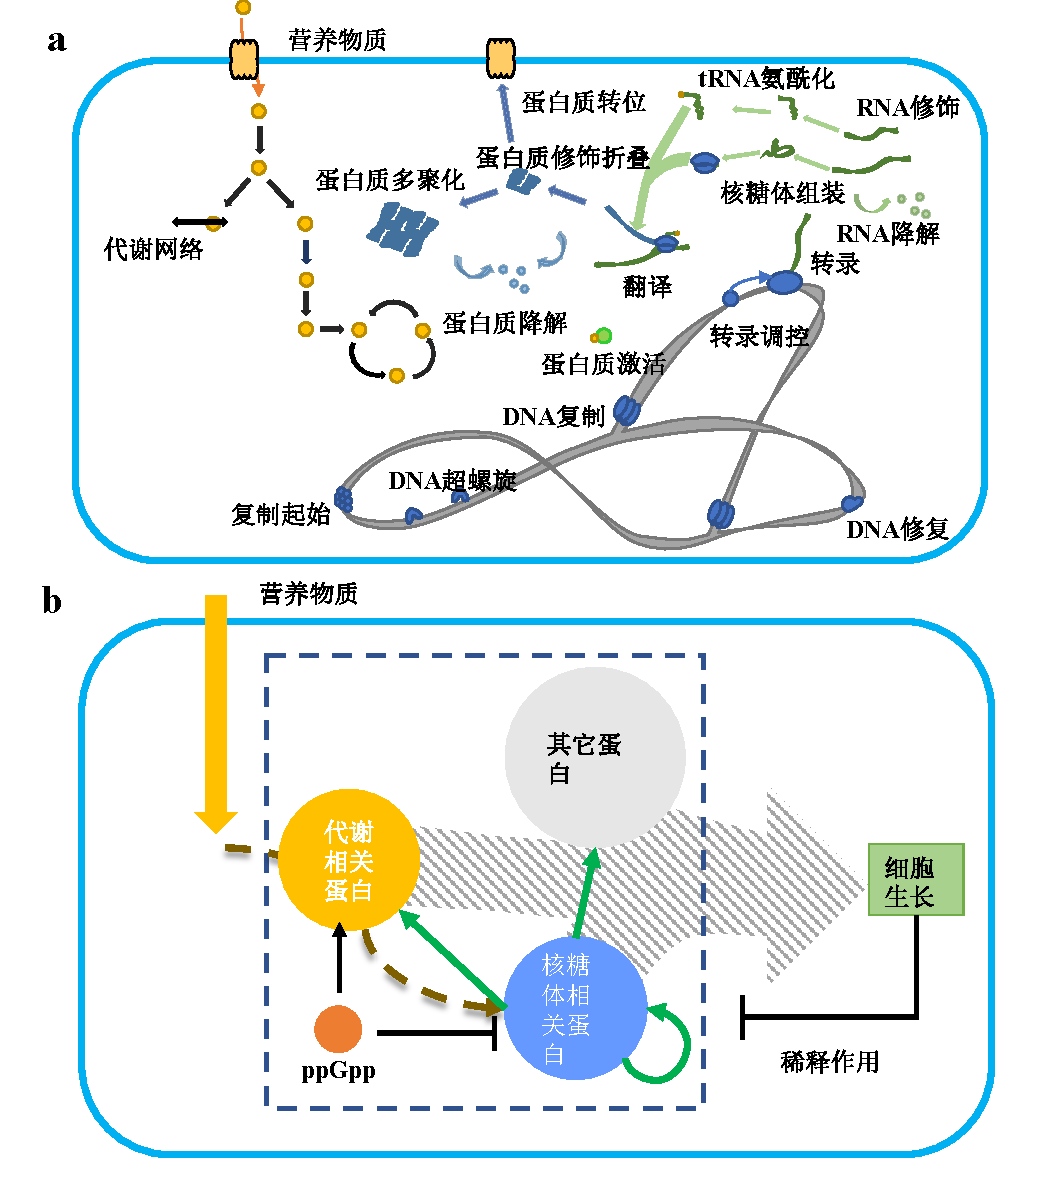
\includegraphics[width=1.0\textwidth]{reviewer_figure2}
  \caption{全细胞模型与粗粒化模型涉及细胞生理过程示意图。{\scriptsize (a)全细胞模型所涉及细胞生理过程,其几乎涵盖了所有已知的生理反应,通过数学手段对每个反应进行描述并整合成28个分区最终合并成完整的细胞模型(图修改自\cite{karr2012whole})(b) 粗粒化模型所涉及细胞生理过程,目前普遍接受的概念是将蛋白质组分成三组:核糖体相关蛋白,代谢相关蛋白和其它蛋白,细胞生长主要是由于蛋白质的增长导致,主要耗能过程为转录及翻译,以ppGpp为代表的调控机制平衡转录翻译所需的前体物质生产和转录翻译速率(图修改自\cite{Liao2017})}}
  \label{fig.2}
\end{figure}
\begin{figure}[H]
  \centering
  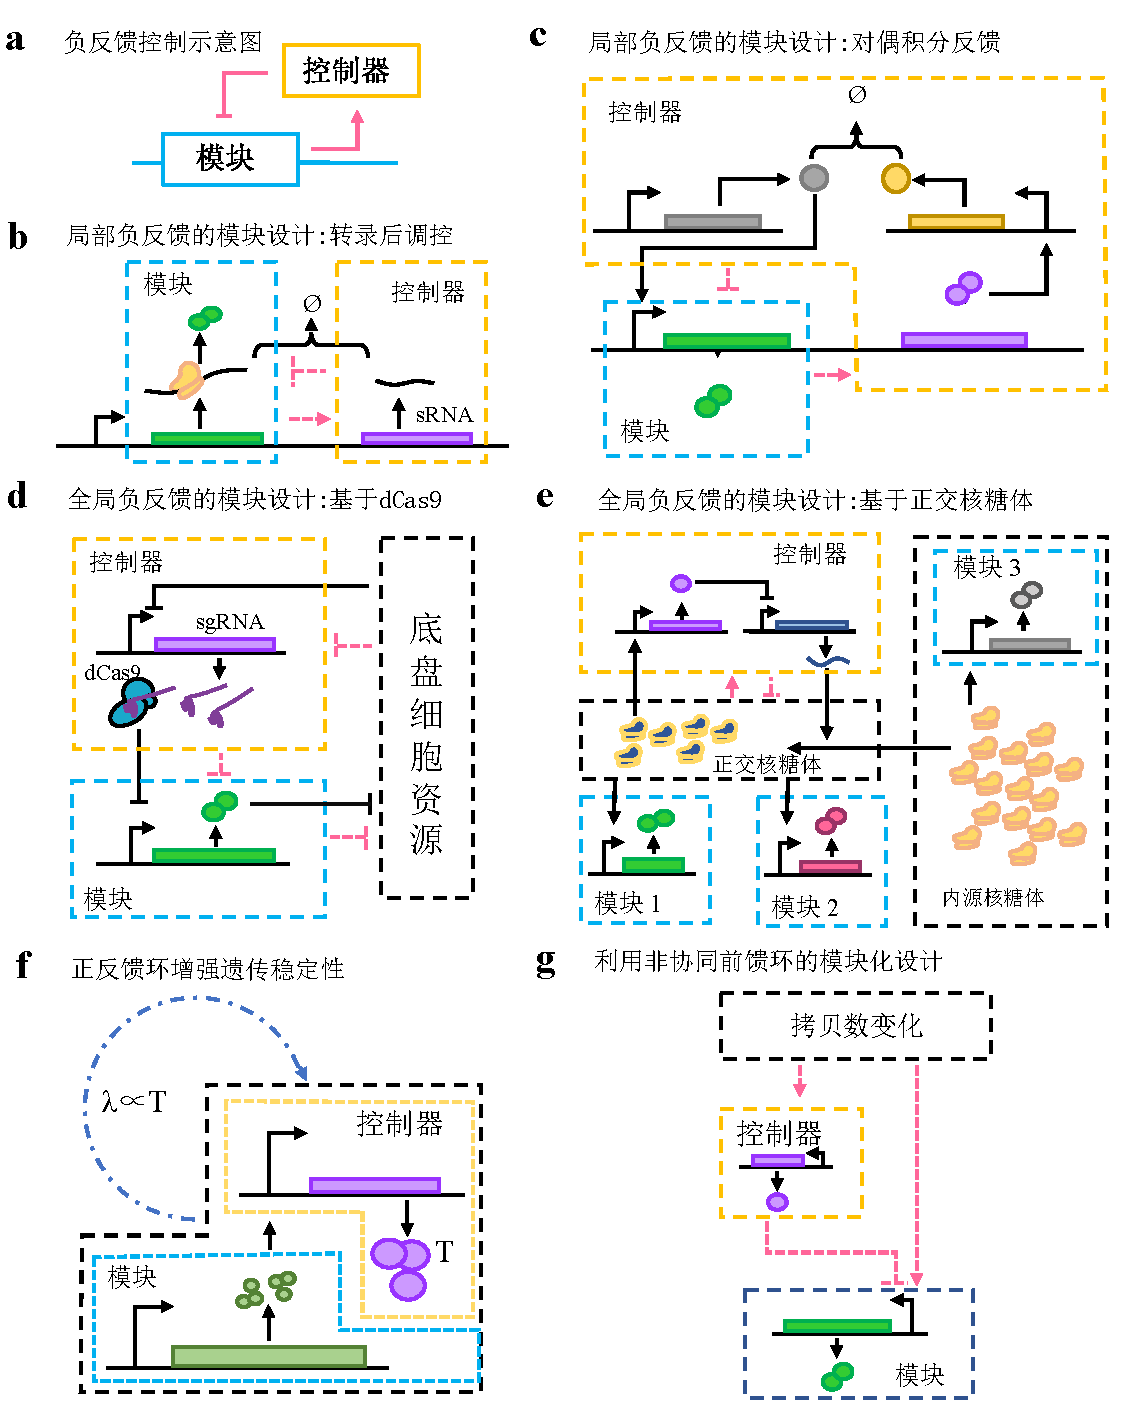
\includegraphics[width=1.0\textwidth]{reviewer_figure3}
  \caption{模块化的基因回路设计。{\scriptsize 更高层次的模块化将基因回路中负责不同功能的局部回路称之为模块,(a)中代表了一个负反馈环,蓝色实线框内代表功能模块,黄色实线框内代表控制器,主要负责调节功能模块,是局部水平负反馈(b、c)的基本模块;基于转录后调控的局部负反馈设计(b),与输出模块一同转录的sRNA是报告基因基因(绿色)序列反义序列,与mRNA结合,引发降解,使报告基因的表达水平与底盘细胞生理解耦合;基于对偶积分反馈的模块化设计(c)则靠控制器内的两个相互拮抗蛋白产物(灰色和黄色)来实现负反馈;全局反馈控制系统(d、e),不同于局部反馈系统,控制器直接感知底盘细胞的资源,(d)中控制器内转录sgRNA的启动子能响应细胞的压力,当模块中外源表达升高时,转录水平上调,sgRNA与胞内组成表达的dCas9蛋白结合,靶向输出模块内的启动子形成负反馈调节;正交翻译系统首先可以将模块3和其余输出模块解耦合,控制器可以稳定正交核糖体(o-ribosome)的胞内浓度,可以给模块1和模块2提供相对充足的翻译资源,一定程度上减轻了模块1和模块2之间对资源的竞争;(f)为生长偶联的正反馈环,输出模块的产物可以激活控制器转录对于底盘而言为关键基因的T,T的表达水平与底盘细胞的生长速度正相关,可以自然淘汰无法或表达过低的个体,增强了遗传稳定性;(g)为利用iFFL设计的可以减少基因拷贝数引起的基因表达水平变化,拷贝数的增加直接使控制器和输出模块的转录水平升高,控制器的产物TALEs蛋白靶向模块内的启动子,由于需要蛋白翻译、成熟等步骤,造成拷贝数的激活作用与TALEs的抑制存在时间差。}}
  \label{fig.3}
\end{figure}

%-------------------------------------------------------------------------%
%    2.8 参考文献
%-------------------------------------------------------------------------%
\vspace{2ex} 
\printbibliography
%为了使参考文献按作者姓氏的拼音排列,使用biblatex里面的caspervector样式,需要使用biber编译,
%编译顺序是XeLatex -> biber -> XeLatex -> XeLatex。

%-------------------------------------------------------------------------%
%    2.9 打印非原创文章的作者信息(作者请忽略此部分)
%-------------------------------------------------------------------------%
\ifthenelse{\equal{\myarticletype}{original}}{}{%
\vspace*{4ex}
\noindent{\kaishu \myfirstauthor}                                       % 第一作者
{\myfirstaffiliation  }                                                   % 第一作者单位
{\myfirstemail   }                                                          % 第一作者email
% \vspace*{1ex}                                                                %如果需要请取消注释
% {\kaishu \mysecondauthor}                                            % 第二作者
% {\mysecondaffiliation }                                                 % 第二作者单位
%{ \mysecondemail }                                                     % 第二作者email
% \vspace*{1ex}                                                           %如果需要请取消注释
% {\kaishu \mythirdauthor}                                              % 第三作者
% \mythirdaffiliation                                                   % 第三作者单位
% \mythirdemail                                                           % 第三作者email
}

%-------------------------------------------------------------------------%
%    2.10 打印责任编辑(作者请忽略此部分)
%-------------------------------------------------------------------------%
% \vspace{4ex}
% \begin{flushright}
% \myeditor
% \end{flushright}

%-------------------------------------------------------------------------%
%    2.11 根据需要打印英文摘要(作者请忽略此部分)
%-------------------------------------------------------------------------%
\ifthenelse{\equal{\mytitleEN}{null}}{}{%
    \newpage
    \printtitlepageEN
}

\end{document}
